\section{Certification}
Goal: given a neural network $N$, a constraint over input $\phi$ and a property over outputs $\psi$, prove that $i \vDash \phi \Rightarrow N(i) \vDash \psi$ or return a violation. We want sound, complete and scalable algorithms, i.e., to either scale sound and complete methods or to make sound but incomplete methods more complete.
\begin{itemize}
    \item If the property does not hold, the program always states the property does not hold.
    \item If the property holds, the program always states the property holds.
\end{itemize}

\subsection*{Convex Relaxations}
Incomplete but sound
\begin{itemize}
    \item Box. Use hypercubes as approximation.
          % \item Zonotope. Represent every variable by $x_i = a^i_0+\sum_j a_j^i \epsilon_j = a_i^T e$, where $\epsilon_i\in [-1,1]$, $a_i\ge 0$. (1) The encoding for affine layer $y=Wx+b$ is $y=W A e+b$, which is exact. (2) To compute the encoding for ReLU layers, we first obtain box bounds by plugging in $\epsilon=-1$ and $\epsilon=1$. When it is strictly positive (negative), then use $y=x$ ($y=0$). For cross-boundary cases, use the line between $(l,0)$ and $(u,u)$ as the upper bound ($y=\lambda(x-l)$, $\lambda=\frac{u}{u-l}$) and its parallel as the lower bound ($y=\lambda x$). Then we compute the standard form of this zonotope by $y = \lambda(x-tl)$, $t\in [0,1]$, plug in $t=(\epsilon_{\text{new}}+1)/2$, $\epsilon_{\text{new}}\in [-1,1]$ and expand.
    \item DeepPoly. Bound every variable by $\sum_j w^l_jx_j + v^l \leq x_i \leq \sum_j w^u_j x_j +v_j$ and $l_i \le x_i \le u_i$. First do a forward propagation and then a backward propagation. (1) For affine layer $y=Wx+b$, use $Wx+b\le y\le Wx+b$. (2) For ReLU layers, if it is strictly positive (negative), use $x\le y\le x$ ($0\le y\le 0$). Otherwise, apply min-area heuristic to choose one from $0\le y\le \lambda(x-l)$ and $x\le y \le \lambda(x-l)$ (where $\lambda=\frac{u}{u-l}$), i.e., choose the first one if $u\leq -l$ o.w. the second one. When forward-propagating, we compute the interval bound by backsubstituting to the first layer.
\end{itemize}

Relaxations of methods not included in one another cannot be compared.

\subsection*{MILP}
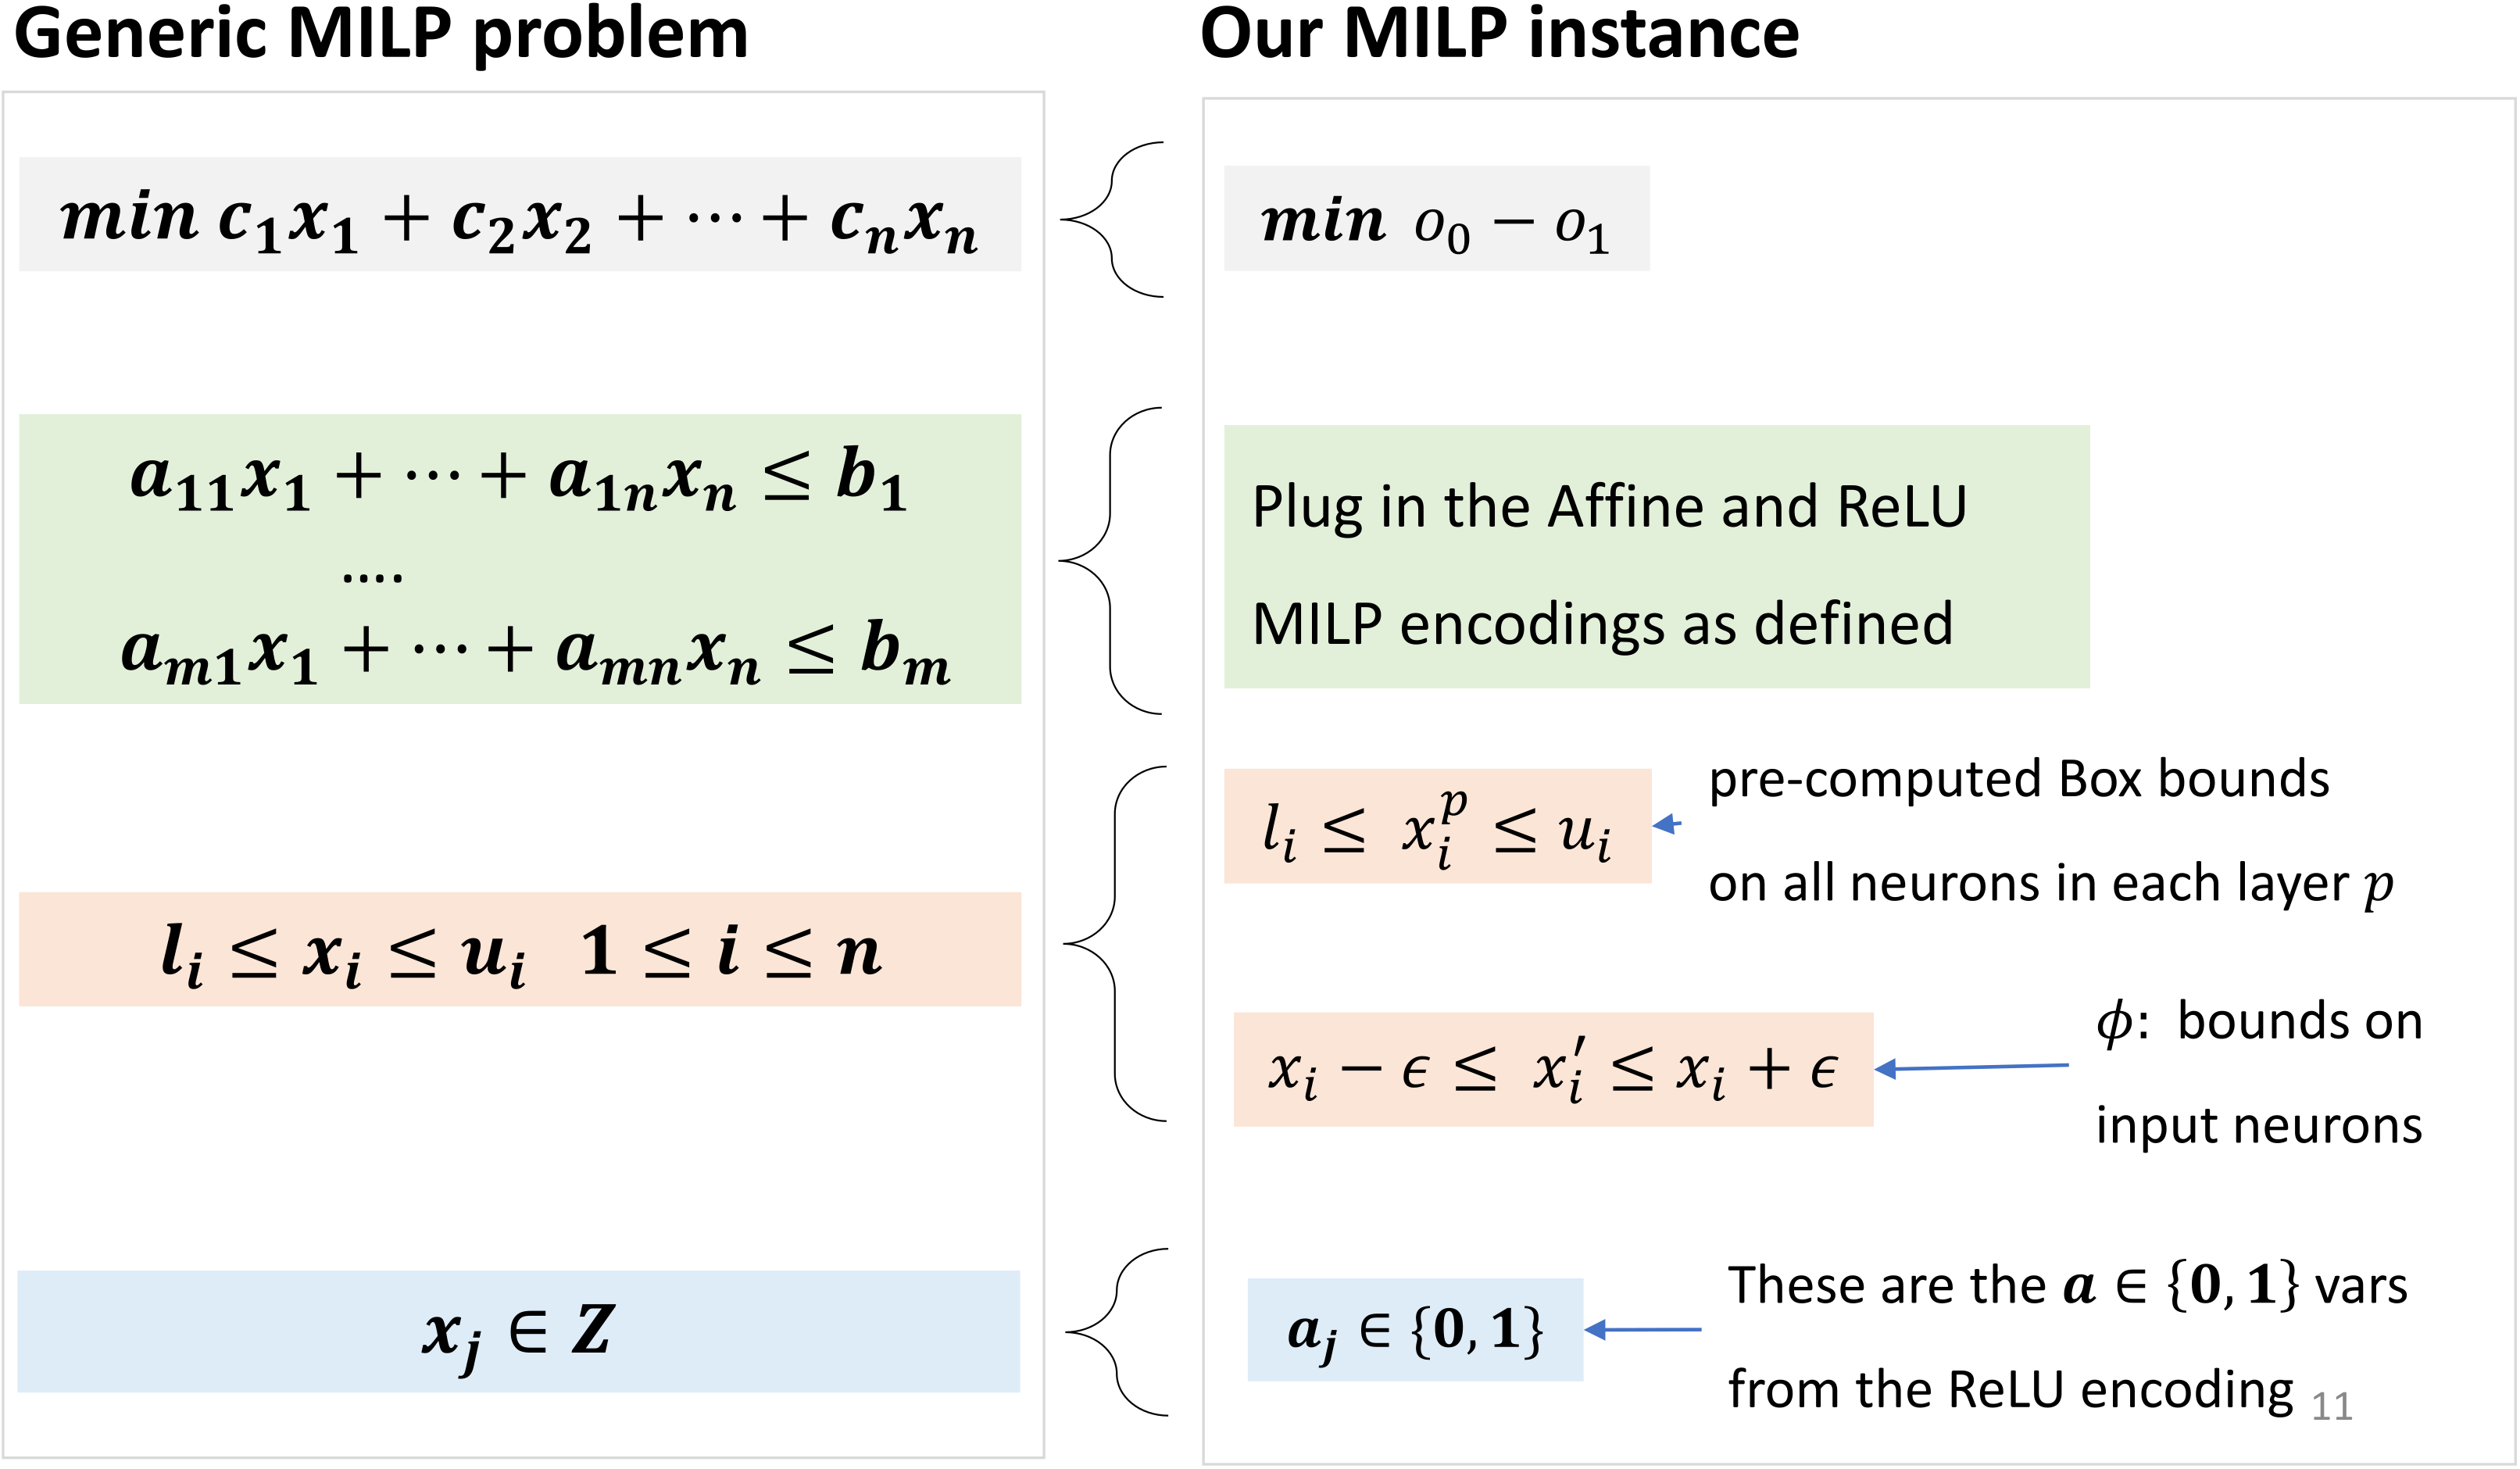
\includegraphics[width=1\linewidth]{img/milp.png}
Complete and sound for ReLU network, but is NP-complete.

The encoding for \textbf{affine} layer is: $Wx+b\le y\le Wx+b$. The encoding for \textbf{ReLU} is: $x\leq y\leq x-l(1-a)$,  $y\le ua$, $y\ge 0$ and $a\in\{0,1\}$. The variable $a$ serves as a ``state'' indicator to encode a piece-wise linear function. The bounds $l,u$ are pre-computed by Box. MILP benefits from Box bounds in that it could stop further exploration of infeasible combinations of integer variables, e.g., if the objective lower bound is positive when $a_1=0$, then there is no need to explore $a_2$ for $a_1=0$.

\subsection*{Branch and Bound}
Can split variables in cases (e.g. \nolinebreak{ReLU} output can be positive or negative) and certify both splits separately. Constraints can be enforced using KKT condition.
% \vspace*{-3mm}
\begin{center}
    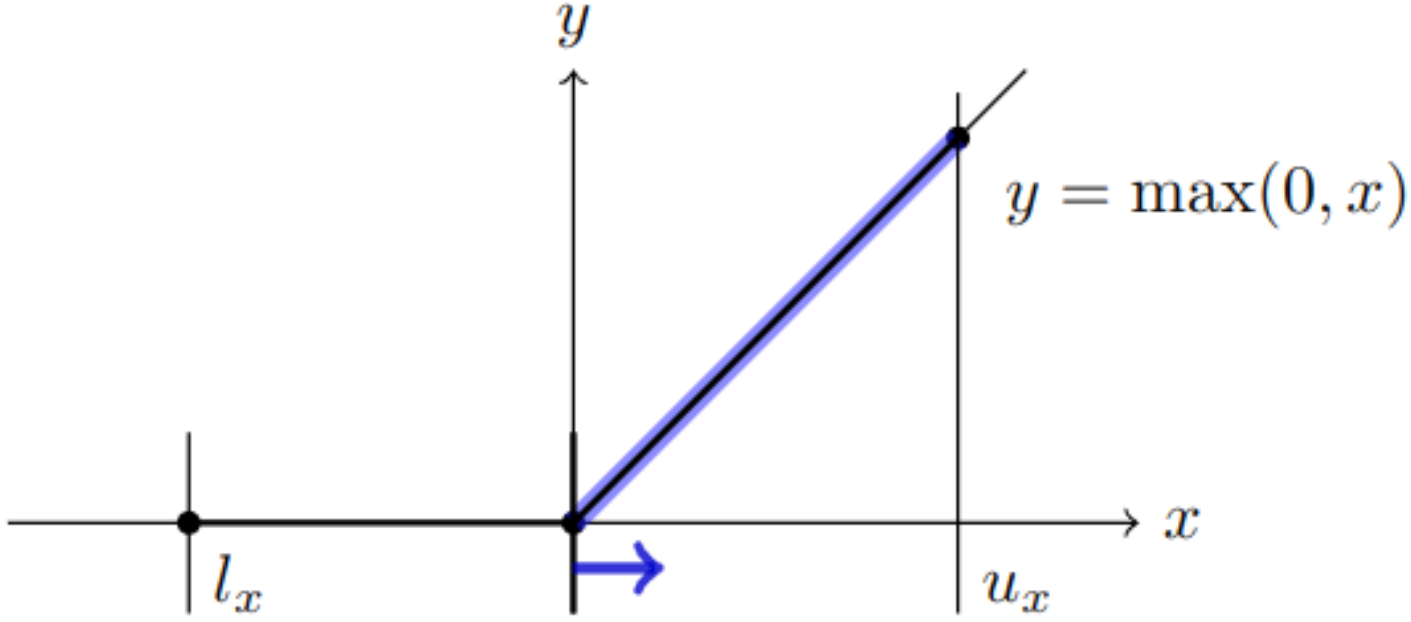
\includegraphics[width=.6\linewidth]{img/bnb.png}
\end{center}
% \vspace*{-2mm}
\begin{equation*}
    \begin{split}
        \max_{x\in\mathcal{X}} \  &a^\top x+c\leq \max_{x\in\mathcal{X}}\min_{\beta\geq0}a^\top x+c+\beta x_i \\[-2mm]
        \text{s.t.} \ \ \        &  x_i\geq0
    \end{split}
\end{equation*}
\Warning Adjust output bounds when splitting.

Initialize queue (without splits). While queue is not empty and not timed out:
1. Get subproblem from queue.
2. Compute bound of interest.
3. If not verified, pick neuron to split according to heuristic.
4. Add both new subproblems to queue.
